\documentclass[tikz, border=5mm]{standalone}

\usepackage{amsmath, amssymb, standalone}
\usetikzlibrary{arrows.meta, positioning, patterns}
\usetikzlibrary{decorations.pathreplacing}
\tikzstyle{box} = [rectangle, rounded corners, 
minimum width=2.5cm, 
minimum height=1cm,
align=center, 
draw=black, 
fill=blue!30]
\tikzstyle{arrow} = [->,thick]


\begin{document}
	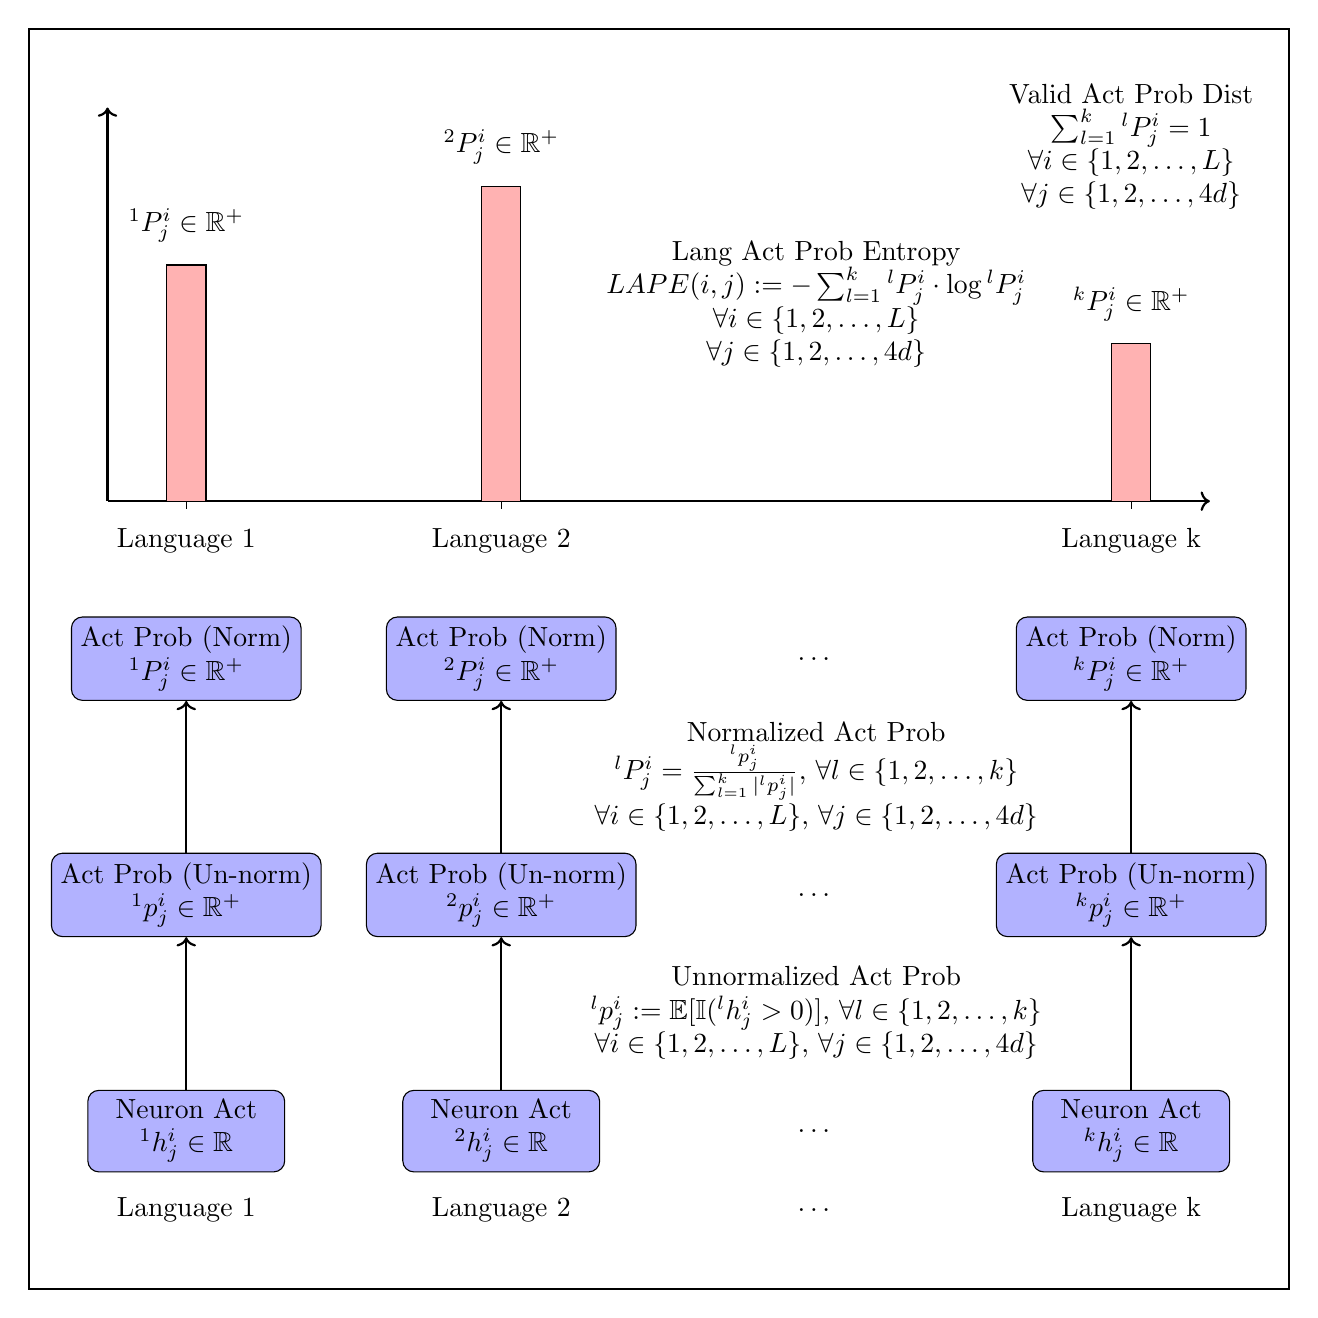
\begin{tikzpicture}
		
		% Define the canvas boundary (optional, for visualization)
		\draw[thick, black] (0,0) rectangle (16,16);
%		\draw[step=1cm,gray,very thin] (0,0) grid (16,16);
		
		\node (l1) at (2,1) {Language 1};
		\node (l2) at (6,1) {Language 2};
		\node (ld) at (10,1) {$\dots$};
		\node (lk) at (14,1) {Language k};
		
		\node[box] (h1) at ([xshift=0cm, yshift=1cm]l1.center) {Neuron Act \\ $^{1}h^{i}_{j} \in \mathbb{R}$};
		\node[box] (h2) at ([xshift=0cm, yshift=1cm]l2.center) {Neuron Act \\ $^{2}h^{i}_{j} \in \mathbb{R}$};
		\node (hd) at ([xshift=0cm, yshift=1cm]ld.center) {$\dots$};
		\node[box] (hk) at ([xshift=0cm, yshift=1cm]lk.center) {Neuron Act \\ $^{k}h^{i}_{j} \in \mathbb{R}$};
		
		\node[align=center] (actprob) at ([xshift=0cm, yshift=1.5cm]hd.center) {Unnormalized Act Prob\\ ${}^{l}p^i_j := \mathbb{E} [\mathbb{I} ({}^l h^i_j > 0)]$, $\forall l \in \{1, 2, \dots, k\}$ \\ $\forall i \in \{1, 2, \dots, L\}$, $\forall j \in \{1, 2, \dots, 4d\}$};
		
		\node[box] (p1) at ([xshift=0cm, yshift=3cm]h1.center) {Act Prob (Un-norm) \\ $^{1}p^{i}_{j} \in \mathbb{R}^+$};
		\node[box] (p2) at ([xshift=0cm, yshift=3cm]h2.center) {Act Prob (Un-norm) \\ $^{2}p^{i}_{j} \in \mathbb{R}^+$};
		\node (pd) at ([xshift=0cm, yshift=3cm]hd.center) {$\dots$};
		\node[box] (pk) at ([xshift=0cm, yshift=3cm]hk.center) {Act Prob (Un-norm) \\ $^{k}p^{i}_{j} \in \mathbb{R}^+$};
		
		\node[align=center] (norm) at ([xshift=0cm, yshift=1.5cm]pd.center) {Normalized Act Prob \\ ${}^l P^i_j = \frac{{}^l p^i_j}{\sum_{l=1}^k |{}^l p^i_j|}$, $\forall l \in \{1, 2, \dots, k\}$ \\ $\forall i \in \{1, 2, \dots, L\}$, $\forall j \in \{1, 2, \dots, 4d\}$};
		
		\node[box] (P1) at ([xshift=0cm, yshift=3cm]p1.center) {Act Prob (Norm) \\ $^{1}P^{i}_{j} \in \mathbb{R}^+$};
		\node[box] (P2) at ([xshift=0cm, yshift=3cm]p2.center) {Act Prob (Norm) \\ $^{2}P^{i}_{j} \in \mathbb{R}^+$};
		\node (Pd) at ([xshift=0cm, yshift=3cm]pd.center) {$\dots$};
		\node[box] (Pk) at ([xshift=0cm, yshift=3cm]pk.center) {Act Prob (Norm) \\ $^{k}P^{i}_{j} \in \mathbb{R}^+$};
		
		
		\draw[thick,->] (1,10) -- (15,10);
		\draw[thick,->] (1,10) -- (1,15);
		\node (x1) at (2,9.5) {Language 1};
		\node (x2) at (6,9.5) {Language 2};
		\node (xk) at (14,9.5) {Language k};
		
		\foreach \x in {2,6,14}
			\draw (\x, 10.1) -- (\x, 9.9);
		
		\filldraw[fill=red!30, draw=black] (1.75,10) rectangle (2.25,13);
		\filldraw[fill=red!30, draw=black] (5.75,10) rectangle (6.25,14);
		\filldraw[fill=red!30, draw=black] (13.75,10) rectangle (14.25,12);
		
		\node (y1) at (2,13.5) {$^{1}P^{i}_{j} \in \mathbb{R}^+$};
		\node (y2) at (6,14.5) {$^{2}P^{i}_{j} \in \mathbb{R}^+$};
		\node[align=center] (yd) at (14,14.5) {Valid Act Prob Dist \\ $\sum_{l=1}^{k} {}^{l}P^{i}_{j} = 1$ \\ $\forall i \in \{1, 2, \dots, L\}$ \\ $\forall j \in \{1, 2, \dots, 4d\}$};
		\node (yk) at (14,12.5) {$^{k}P^{i}_{j} \in \mathbb{R}^+$};
		
		\node[align=center] (lape) at (10,12.5) {Lang Act Prob Entropy \\ $LAPE(i, j) := - \sum_{l=1}^{k} {}^{l}P^{i}_{j} \cdot \log {}^{l}P^{i}_{j}$ \\ $\forall i \in \{1, 2, \dots, L\}$ \\ $\forall j \in \{1, 2, \dots, 4d\}$};
		
		\draw[arrow] (h1) -- (p1);
		\draw[arrow] (h2) -- (p2);
		\draw[arrow] (hk) -- (pk);
		
		\draw[arrow] (p1) -- (P1);
		\draw[arrow] (p2) -- (P2);
		\draw[arrow] (pk) -- (Pk);

		
%		% Edges
%		\draw[arrow] (input) -- (selfattn);
%		\draw[arrow] (selfattn) -| (W1);
%		\draw[arrow] (selfattn) -| (W3);
%		\draw[arrow] (W1) -- (silu);
%		\draw[arrow, red, ultra thick] (silu) |- node[anchor=south, align=center, black] {$\mathbf{h}^i \in \mathbb{R}^{T \times d}$ \\ $h^i_j$: $j^{th}$ Neuron of $i^{th}$ Layer \\ ($\forall j \in \{1, 2, \dots, 4d\}$)} (mult);
%		\draw[arrow] (W3) |- (mult);
%		\draw[arrow] (mult) -- (W2);
%		\draw[arrow] (W2) -- (output);
%		
%		\draw [decorate, decoration={brace, amplitude=20pt}, thick]
%		(2, 2) -- (2, 12) 
%		node[midway, xshift=-1.25cm, rotate=90] {$i^{th}$ MLP Layer ($\forall i \in \{1, 2, \dots, L\}$)};
		
	\end{tikzpicture}
	
\end{document}